\chapter{Estudo da conservação da energia}

\vspace{-0.5cm}

Neste experimento vamos estudar a conservação da energia mecânica de um sistema formado por um carrinho de massa $M$, uma polia de massa desprezível, um fio também de massa desprezível e inextensível, e um corpo de massa $m$, como se mostra na Figura~\ref{fig:energia}.

Tendo em conta que não existe atrito entre o carrinho de massa $M$, nem entre o fio e a polia, mostre que a aceleração do sistema será
\begin{equation}
a = \frac{m g}{ m + M}.
\end{equation}
\noindent

Escreva as equações de energia mecânica do sistema antes que a massa $m$ alcance o chão. Que movimento realiza a massa $M$ depois de a massa $m$ alcançar o chão?

\begin{figure}[h]
\vspace{-0.2cm}
\begin{center}
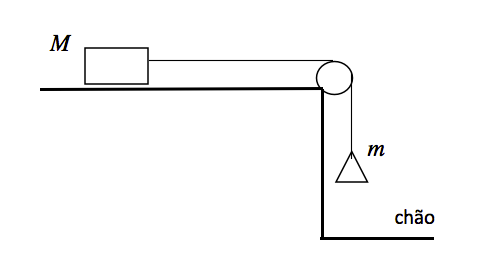
\includegraphics[width=10cm]{fig/EnergiaEsquema}
\caption{\label{fig:energia} Desenho experimental.}
\vspace{-0.5cm}
\end{center}
\end{figure}


\section*{Processo Experimental}

\begin{num}
\item Certifique-se de que o trilho de ar e o sistema de aquisição de dados estejam funcionando corretamente. Caso contrário, ajuste os parâmetros necessários. 
\item Com a ajuda de uma balança, determine a massa do carrinho ($M$) e a do corpo amarrado a ele ($m$). A massa deste corpo deve estar entre 10 g e 30 g.
\item Montar o experimento seguindo a Figura~\ref{fig:energia}.
\item Soltar o corpo de massa $m$ de uma altura $h_0$, submetendo desta forma o carrinho a uma aceleração.

\underline {Importante:} 
Antes de realizar a tomada de dados pensar como irão registrar, além do movimento do carrinho, a posição da massa $m$ em cada instante. Discuta com seu professor. 

\item Pense como identificar ou marcar no vídeo o momento em que a massa $m$ toca o chão.  Discuta com seu professor.

\item Uma vez que saibam as medidas que deverão ser feitas, proceder à tomada de dados.
\end{num} 


\vspace{-0.5cm}
\section*{Levantamento de dados}

\begin{num}
\item Calibre a sua imagem.
\item Construa uma tabela para cada massa de posição em função do tempo, com pelo menos 10 pontos antes e 10 pontos depois do impacto da massa $m$ no chão. Da mesma forma que no Experimento~\ref{g} utilize intervalos de tempo constantes. 
\end{num}

\vspace{-0.5cm}
{\bf Observação:} O aluno pode escolher o método a utilizar para o levantamento dos dados: Leitura Manual ou Leitura Automatizada (Apêndice~\ref{image}).



\section*{Análise de dados}
\subsection*{Parte I: Estudo cinemático do movimento}

\begin{num}
\item Calcule, para cada massa, as velocidades instantâneas com suas respectivas incertezas.
\item Grafique, para a massa $M$, a posição e velocidade em função do tempo (com suas respectivas incertezas quando for possível). 
\item A partir do ajuste linear do gráfico de velocidades da massa $M$, calcule a aceleração e comparé-na com o modelo teórico.
\item Determine os valores de velocidade inicial e final da massa $M$.
\item Determine, a partir das equações de velocidade, o tempo crítico $t_c$, tempo no qual a massa $M$ passa de movimento acelerado a constante. Marque este tempo nos de gráficos posição e velocidade. 

\end{num}
\noindent
\vspace{-1.5cm}
\subsection*{Parte II: Conservação da energia}

\begin{num}
\setcounter{enumi}{7}

\item Na região na qual o movimento é acelerado, estudar a conservação da energia. Para isto construa uma tabela de energias do sistema constituído pelo carrinho, corpo, polia e fio. A tabela deve conter as seguintes informações: tempo, energia cinética total, energia potencial gravitacional total (pensar onde é conveniente colocar o sistema de referência para facilitar o cálculo), energia mecânica total. 
\item Faça um gráfico que contenha a energia cinética, potencial e mecânica em função do tempo.
\item Discuta a partir do gráfico obtido, se há ou não conservação da energia mecânica. Justificar.
\item Qual é o valor da energia mecânica do sistema na região na qual o movimento é acelerado? O que acontece com a energia mecânica na outra região?
\end{num}

{\bf Observação:}
\vspace{-0.5cm}
\begin{iten}
\item A aceleração da gravidade no Rio de Janeiro é $g = (978,7 \pm 0,1)$ cm/s$^2$.  
\item Não esqueça colocar todos os cálculos de propagação de incerteza num Apêndice. 
\end{iten}


\vspace{-0.7cm}
\section*{Opcional}

\begin{num}
\item Obtenha experimentalmente o valor obtido para a aceleração em cada ponto com suas respectivas incertezas e compare o valor de aceleração encontrado com o obtido com o ajuste linear.  Que pode concluir?
\item Realize um gráfico de aceleração em função do tempo para os dois métodos em que a aceleração foi determinada. Discuta.
\end{num}




